\chapter{Работни среди}

Блоковите програмни езици са подразделение на визуалните програмни езици. Същината на блоковите езици е, че програмните инструкции се въвеждат под формата на цветни блокове, а не както е в класическите програмни езици, чрез изписване на текстови команди. Най-основната цел на блоковите езици е да направят областта програмиране значително по-достъпна за начинаещите. Тази цел се постига чрез три основни направления. От синтактична гледна точка, инструкциите в блоковите езици са под формата на цветни иконки. Това значително намалява възможността за изписването на грешна програмна инструкция. На второ място се подобрява семантиката, като всяка от възможните програмни инструкции е добре документирана. На трето място е прагматизма, който позволява изучаването на различните състояния в които може да изпадне програмата. Програмните среди за блоково програмиране набират все по-голяма популярност през последното десетилетие. Някои от най-популярните са: Scratch, Blockly, App Inventor for Android, Ardublock и други. В тази книга ще се спрем на две от програмните среди за блоково програмиране, създадени в Масачузетския технологичен институт, Scratch и App Inventor for Android. Причината за този избор е, че Scratch има насоченост към най-малките, а именно децата в началните училищни класове, което много добре се съчетава с възможностите блоковите програми да бъдат визуализирани и на мобилен телефон, чрез App Inventor for Android. И при двете програмни среди не се изисква инсталирането на специализиран софтуер. Достатъчно е наличието на съвременен компютър, свързан в Интернет и съвременна версия на уеб браузър. 

\section{Първи стъпки в Sratch}

Работата в средата на Sratch започва със зареждане на главната уеб страница (Фиг. \ref{fig0001}), която се намира на адрес: \\ \href{https://scratch.mit.edu/}{https://scratch.mit.edu/}

\begin{figure}[H]
  \centering
  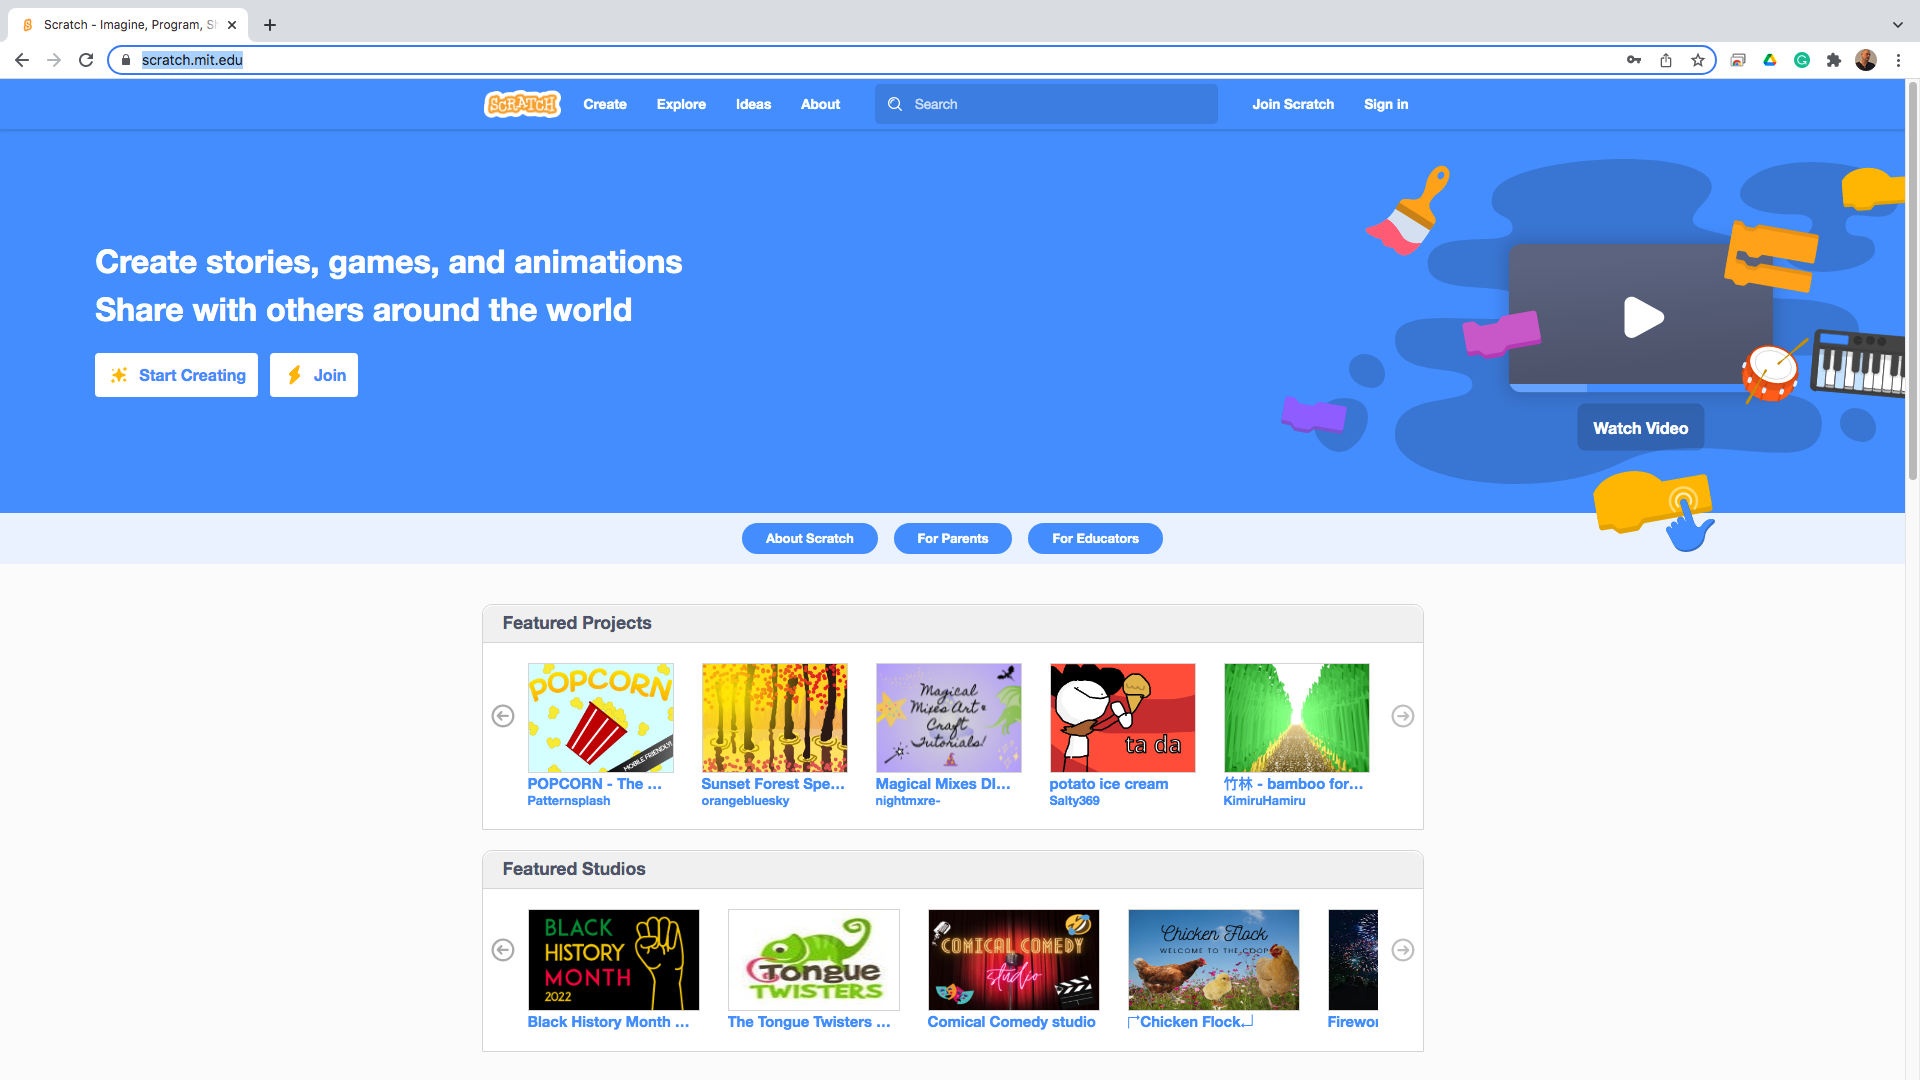
\includegraphics[width=1.0\linewidth,height=0.5\linewidth]{fig0001.png}
  \caption{Начална уеб страница на Sratch}
\label{fig0001}
\end{figure}

Програмната среда на Sratch е организирана на принципа на облачните услуги. Поради тази причина, всеки желаещ да използва услугата трябва да си направи регистрация (Фиг. \ref{fig0002}). Регистрацията се състои от потребителско име и парола.

\begin{figure}[H]
  \centering
  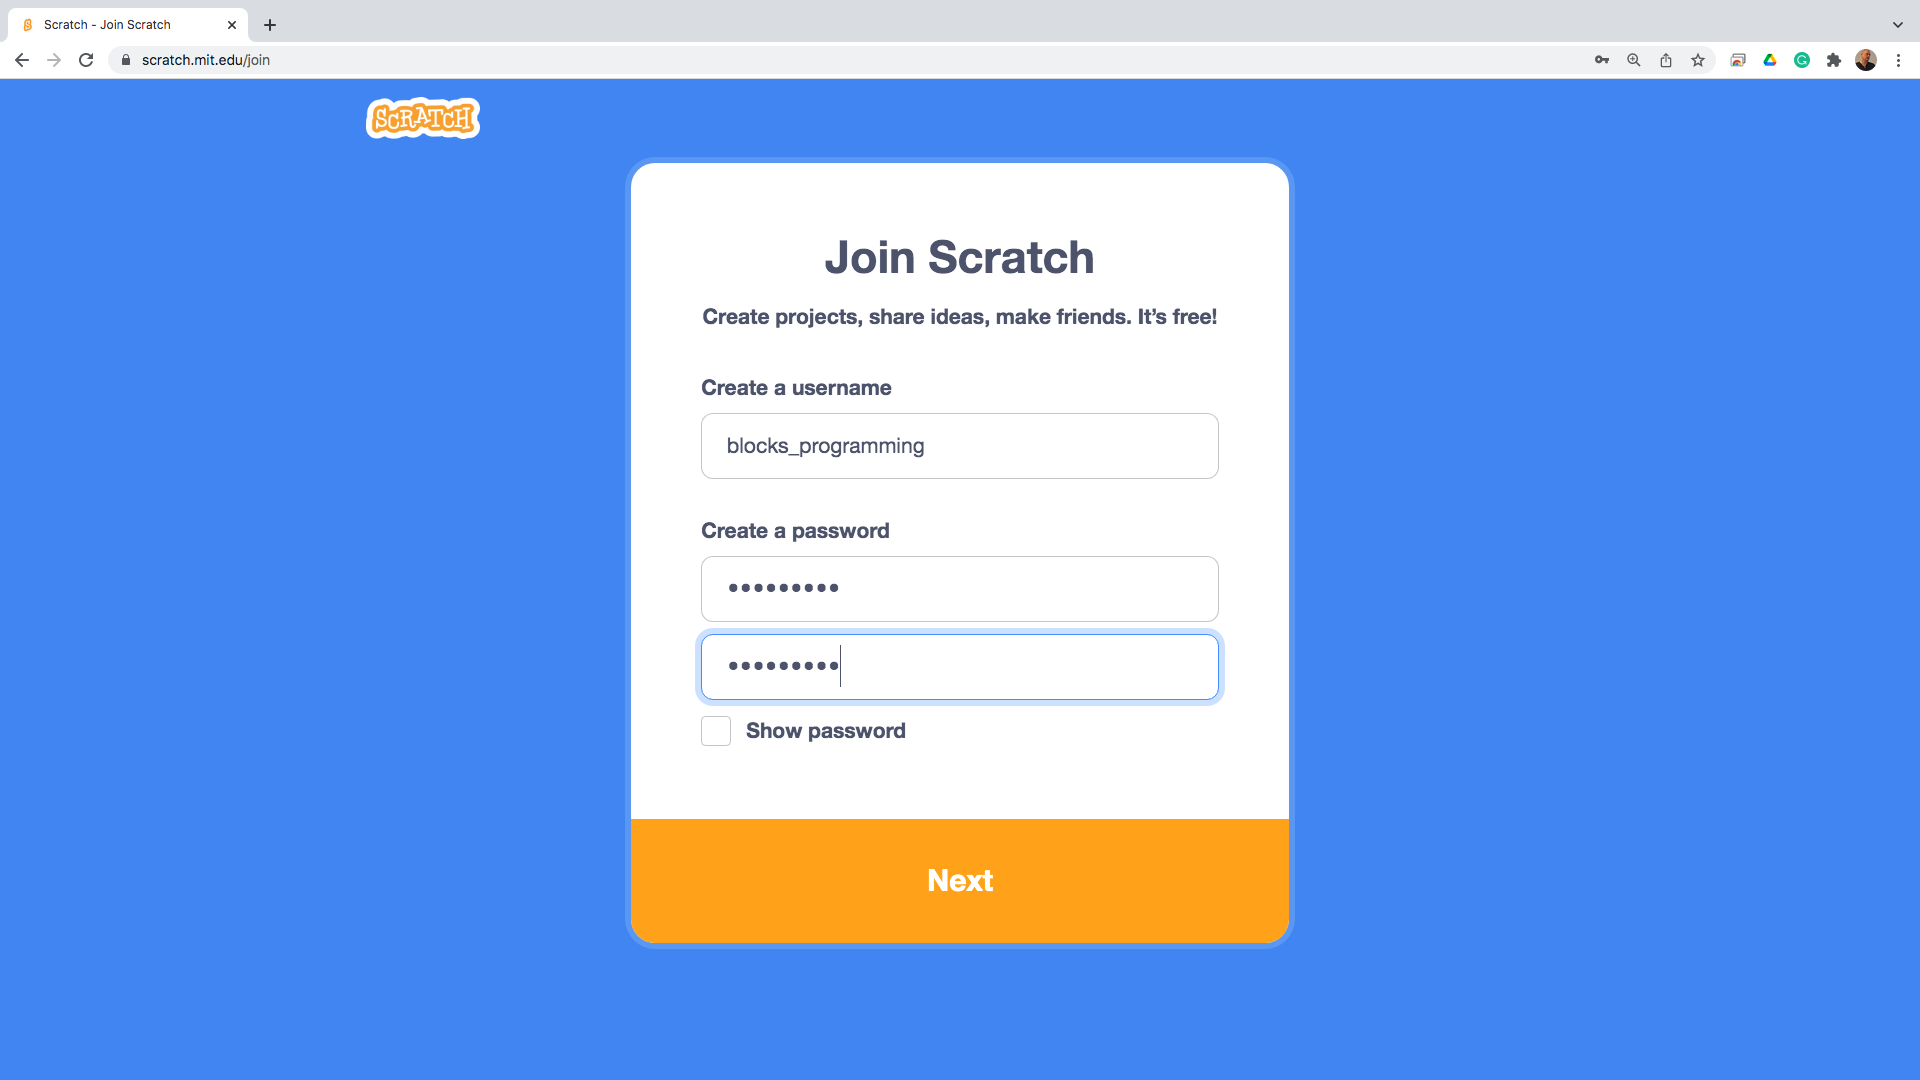
\includegraphics[width=1.0\linewidth,height=0.5\linewidth]{fig0002.png}
  \caption{Регистрация на потребител в Sratch}
\label{fig0002}
\end{figure}

След избора на потребителско име и парола следва определяне на географския регион в който се намира потребителят (Фиг. \ref{fig0003}).

\begin{figure}[H]
  \centering
  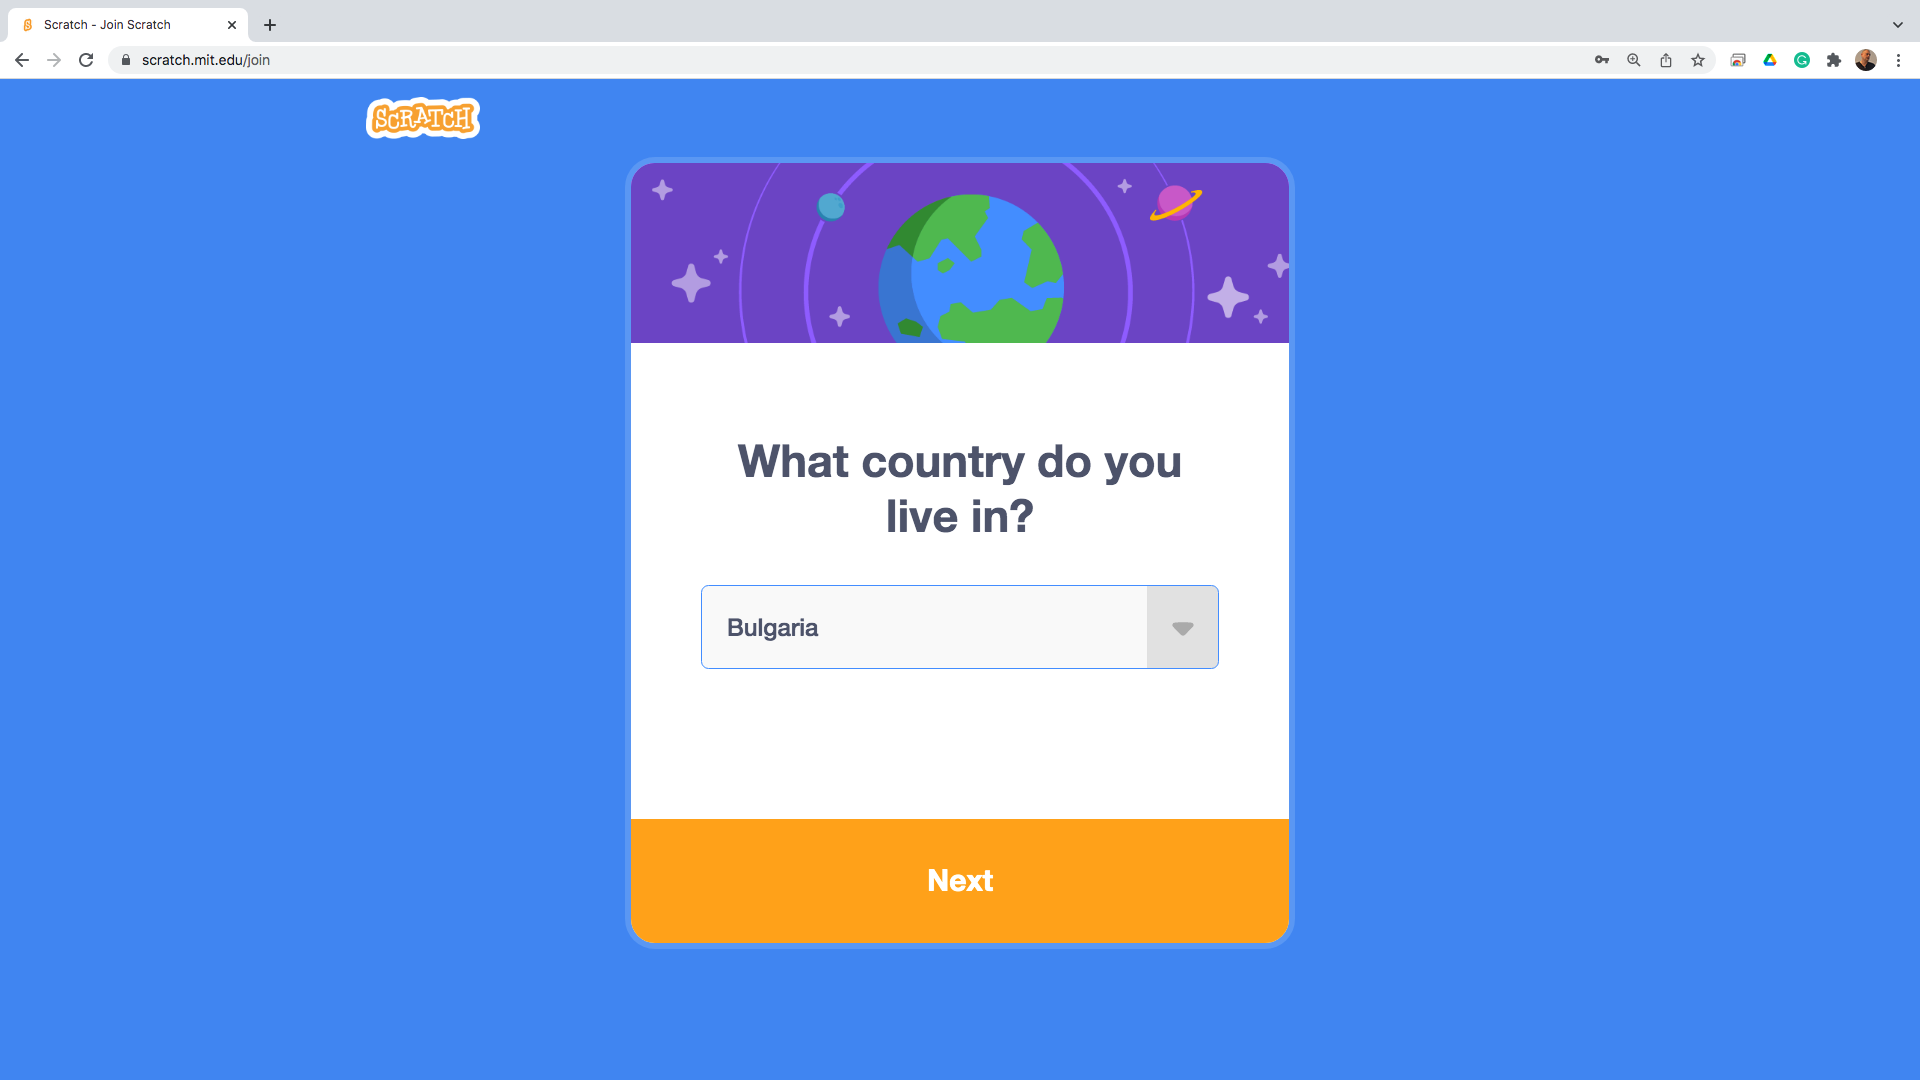
\includegraphics[width=1.0\linewidth,height=0.5\linewidth]{fig0003.png}
  \caption{Географско местоположение}
\label{fig0003}
\end{figure}

Платформата е насочена предимно към деца, изразяващи интерес към програмирането, но също така към родители и учители. Поради тази причина, системата събира информация за възрастта на потребителя (Фиг. \ref{fig0004}).

\begin{figure}[H]
  \centering
  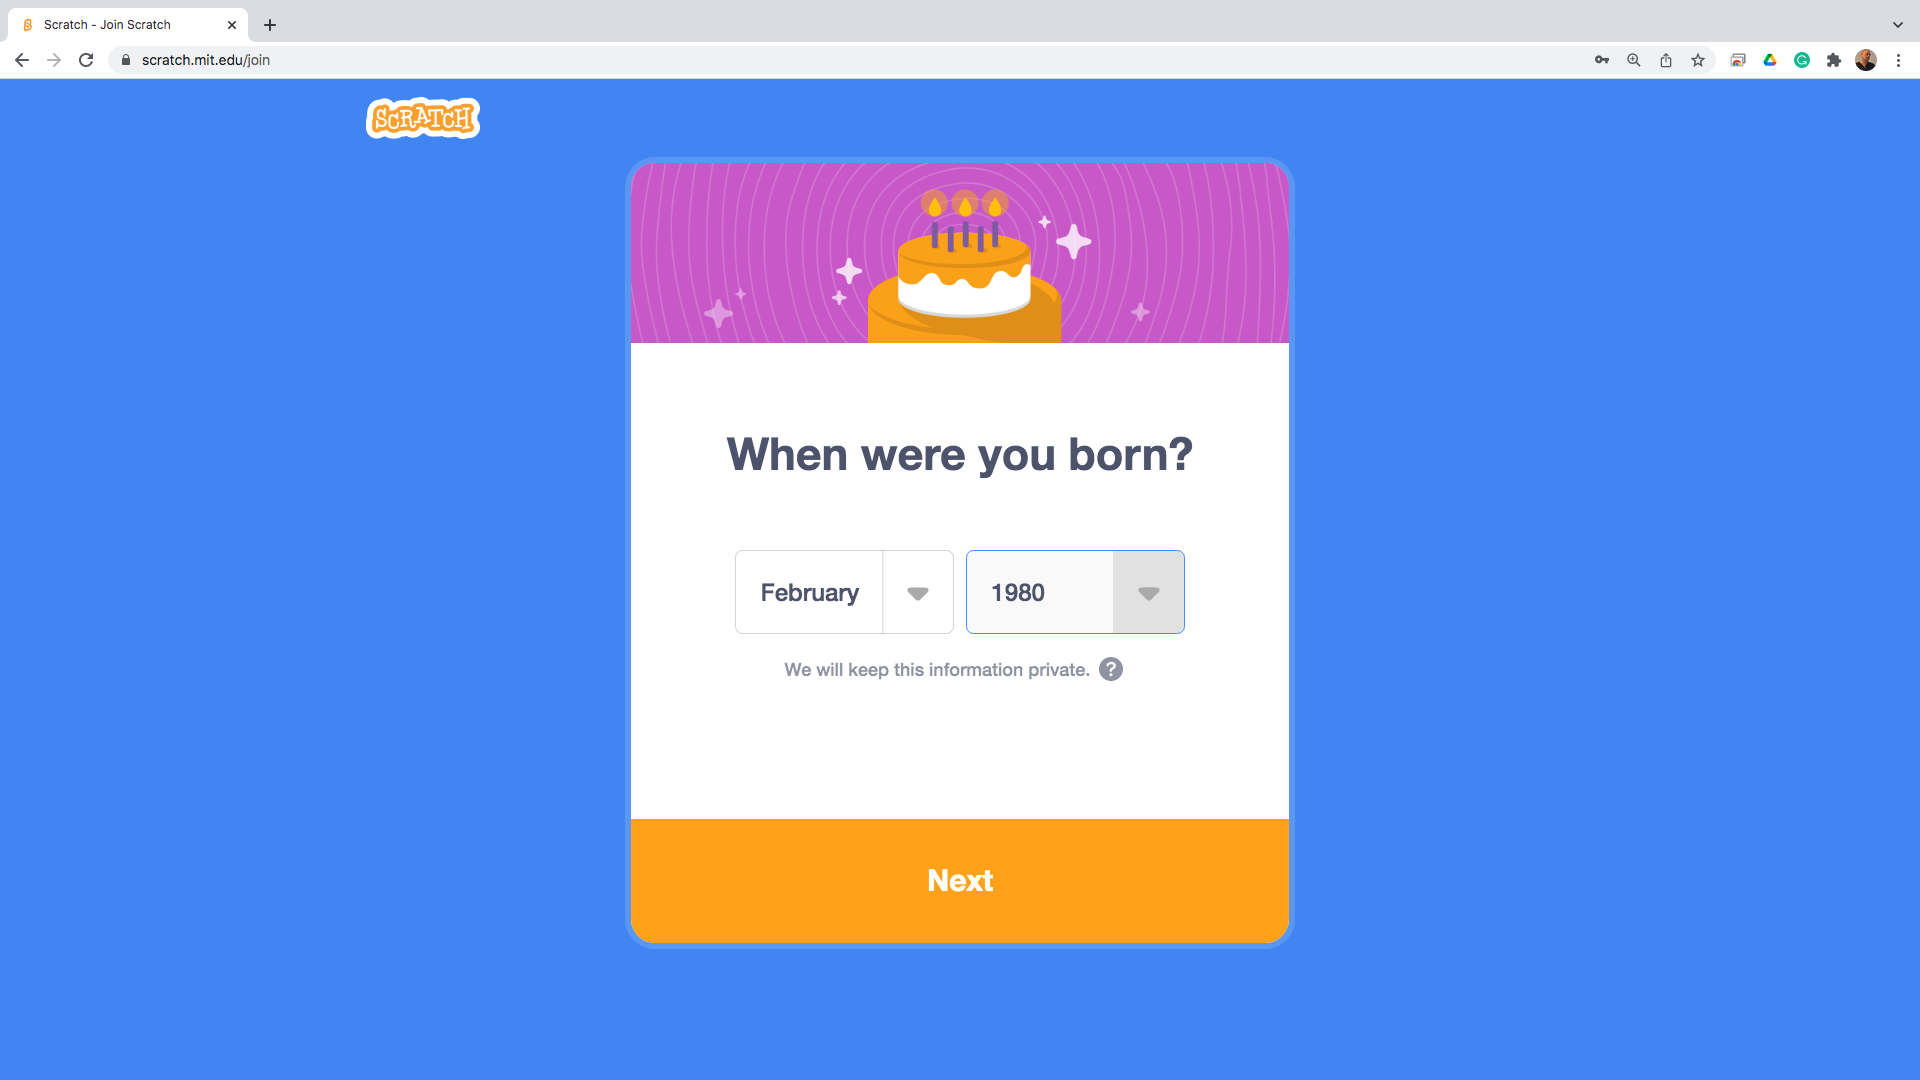
\includegraphics[width=1.0\linewidth,height=0.5\linewidth]{fig0004.png}
  \caption{Възраст на потребителя}
\label{fig0004}
\end{figure}

Освен класификация по възраст, системата събира информация и за класификация по полова принадлежност. Тази информация е незадължителна, основно за да не бъде дискриминираща (Фиг. \ref{fig0005}).

\begin{figure}[H]
  \centering
  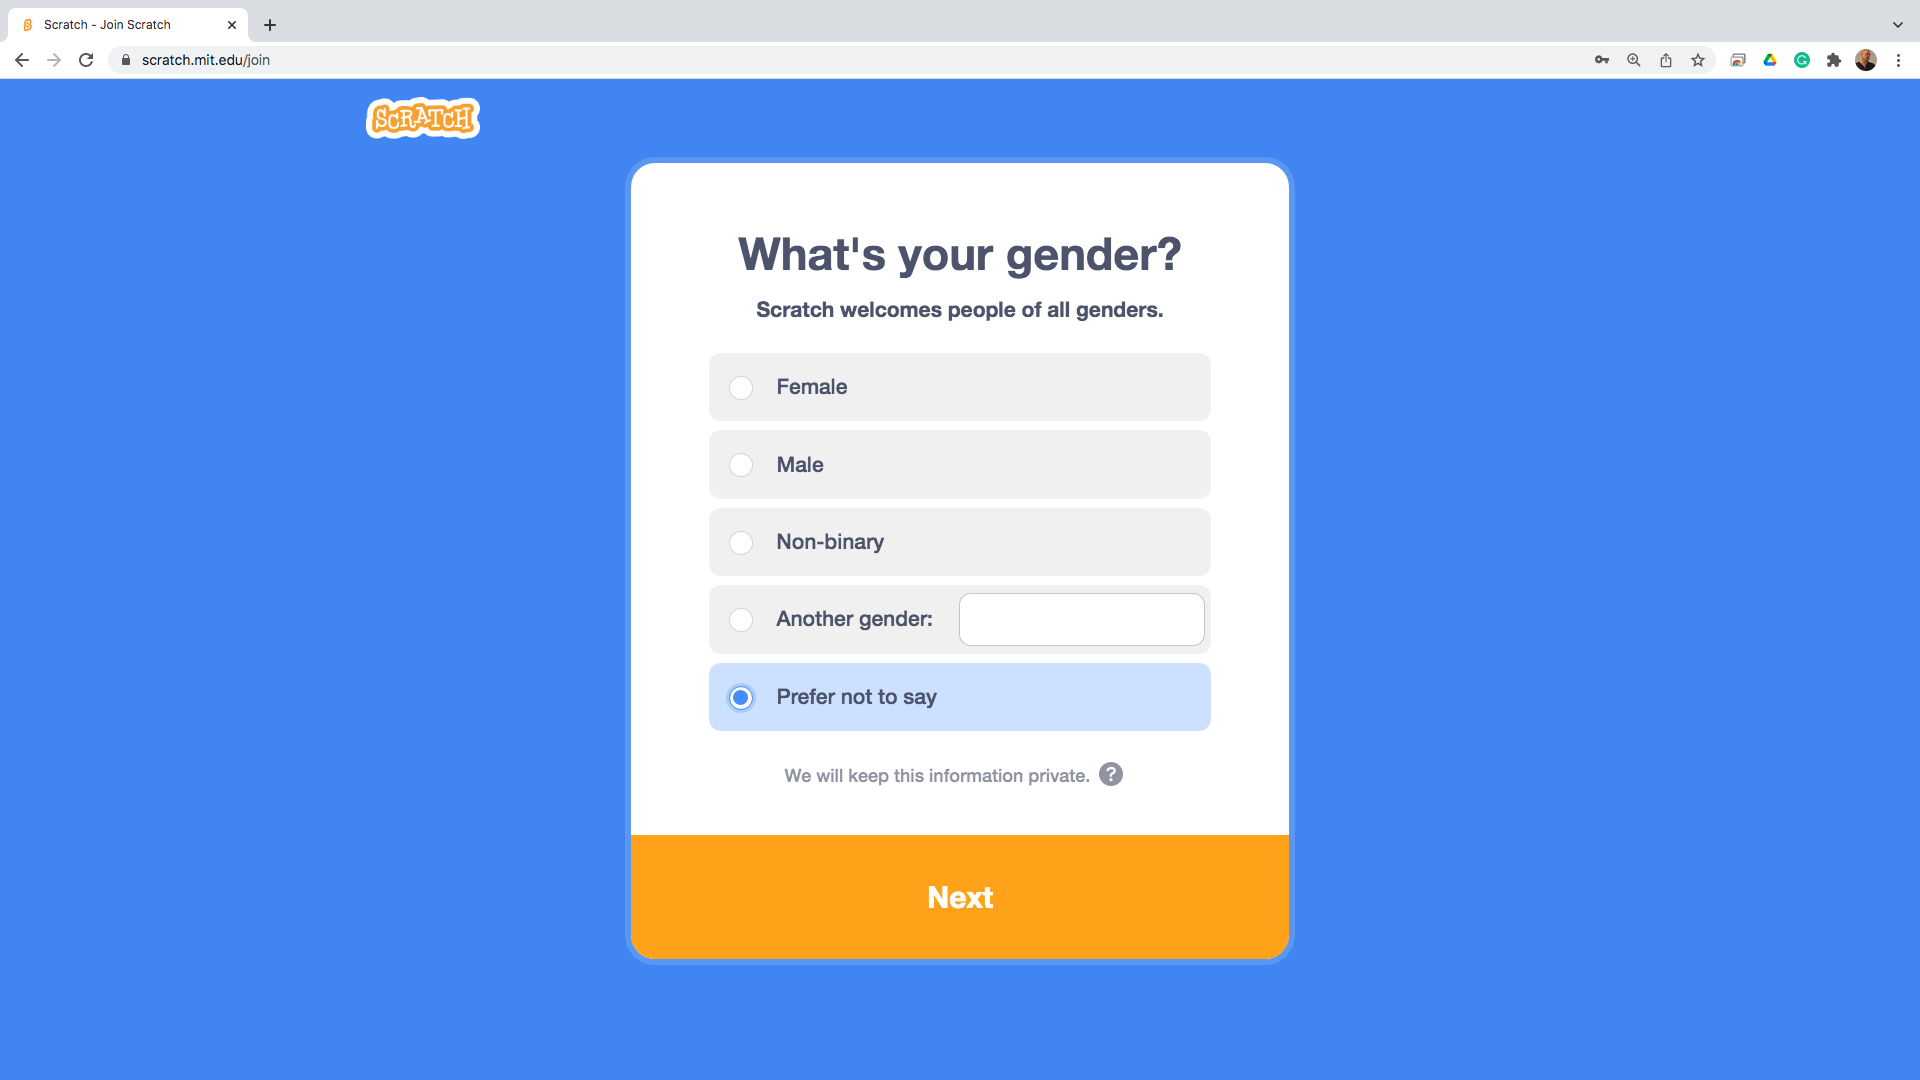
\includegraphics[width=1.0\linewidth,height=0.5\linewidth]{fig0005.png}
  \caption{Пол на потребителя}
\label{fig0005}
\end{figure}

Потребителският профил, освен с потребителско име и парола, трябва да бъде аоцииран и с адрес на електронна пощенска кутия (Фиг. \ref{fig0006}).

\begin{figure}[H]
  \centering
  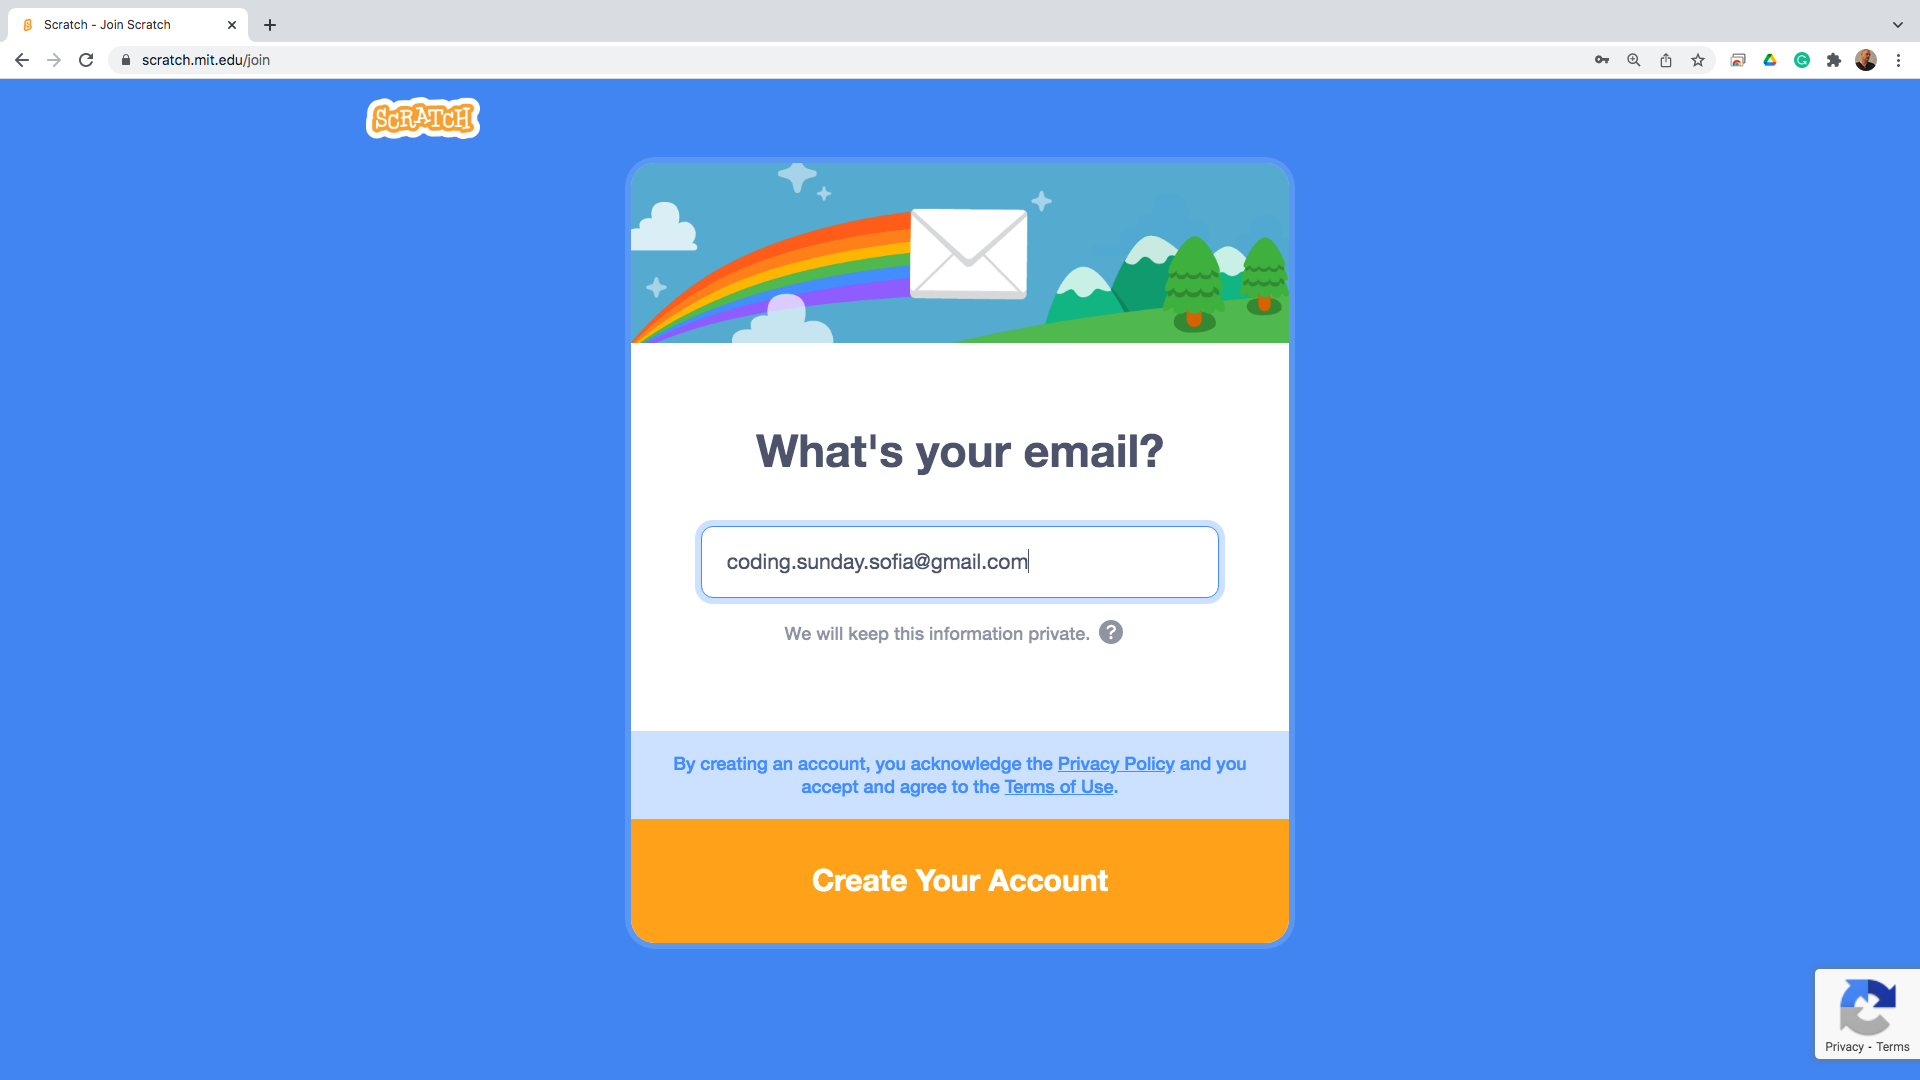
\includegraphics[width=1.0\linewidth,height=0.5\linewidth]{fig0006.png}
  \caption{Адрес на електронна поща на потребителя}
\label{fig0006}
\end{figure}

Процесът по регистрация на потребител в системата е почти завършен (Фиг. \ref{fig0007}). Остава само стъпката за потвърждаване на избрания адрес за електронна поща.

\begin{figure}[H]
  \centering
  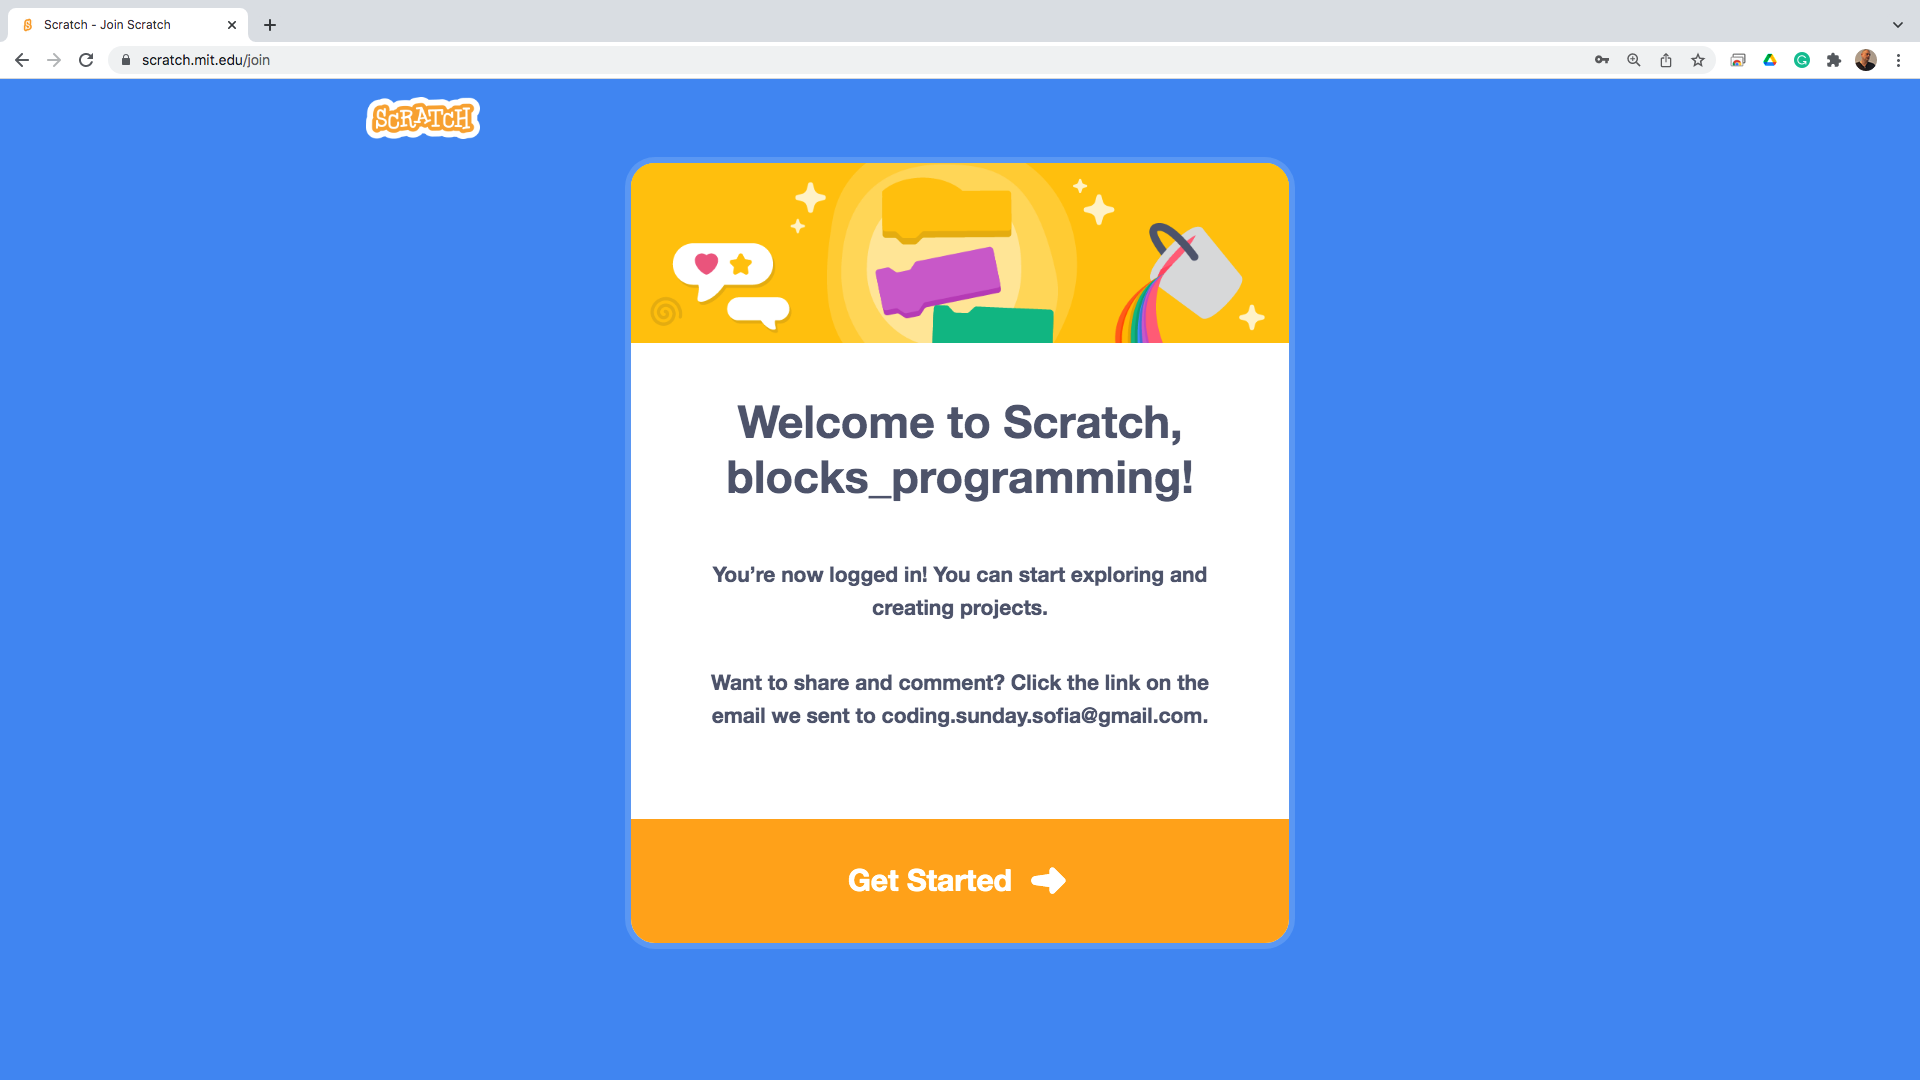
\includegraphics[width=1.0\linewidth,height=0.5\linewidth]{fig0007.png}
  \caption{Приключване на процеса за въвеждане на информация за потребителя}
\label{fig0007}
\end{figure}

Електронното писмо, за потвърждаване на потребителската регистрация, съдържа електронна препратка до уеб сайта на Sratch (Фиг. \ref{fig0008}). Тази препратка трябва да бъде последвана за да се завърши процесът по регистрация на нов потребител. 

\begin{figure}[H]
  \centering
  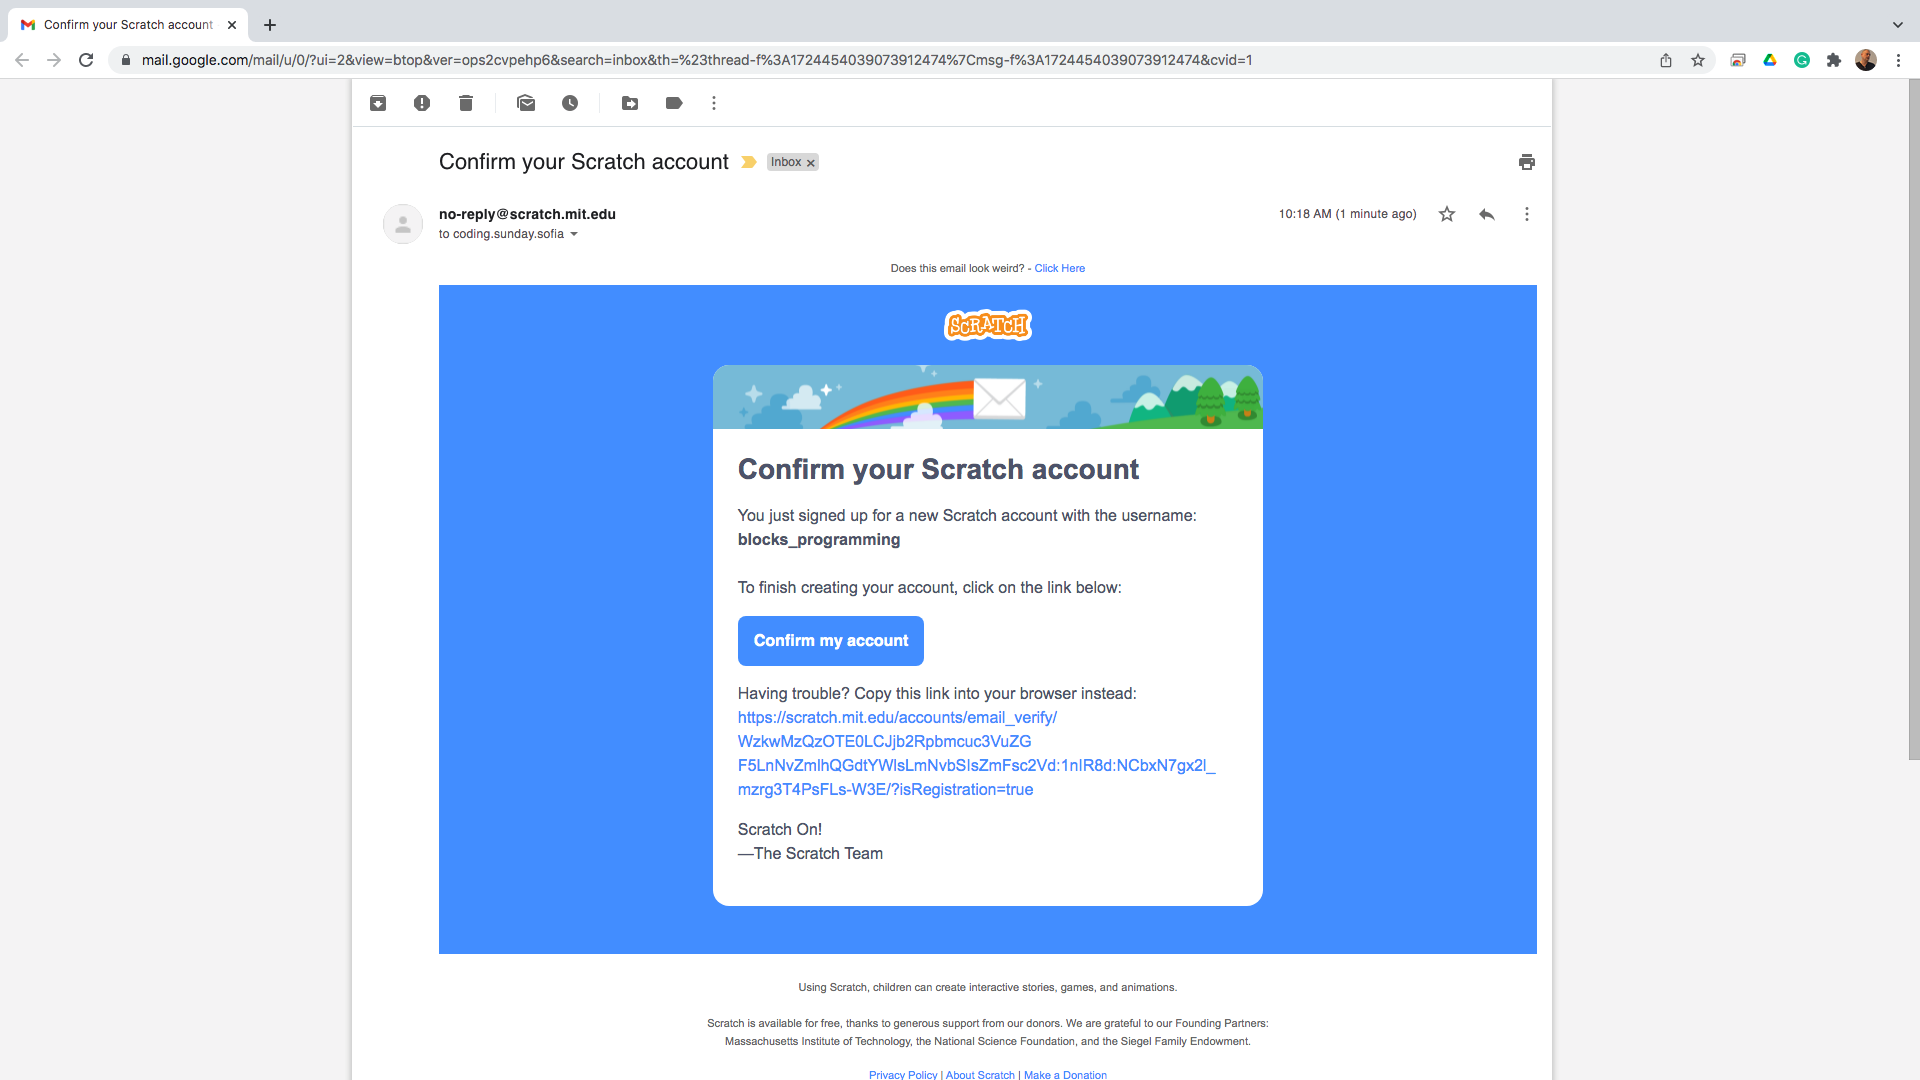
\includegraphics[width=1.0\linewidth,height=0.5\linewidth]{fig0008.png}
  \caption{Електронно съобщение за потвърждаване на електронния адрес}
\label{fig0008}
\end{figure}

Регистрацията на новия потребител приключва със зареждането на начален работен екран (Фиг. \ref{fig0009}). Горе, в дясно се вижда изписано потребителското име, избрано на първата стъпка от процеса по регистрацията.

\begin{figure}[H]
  \centering
  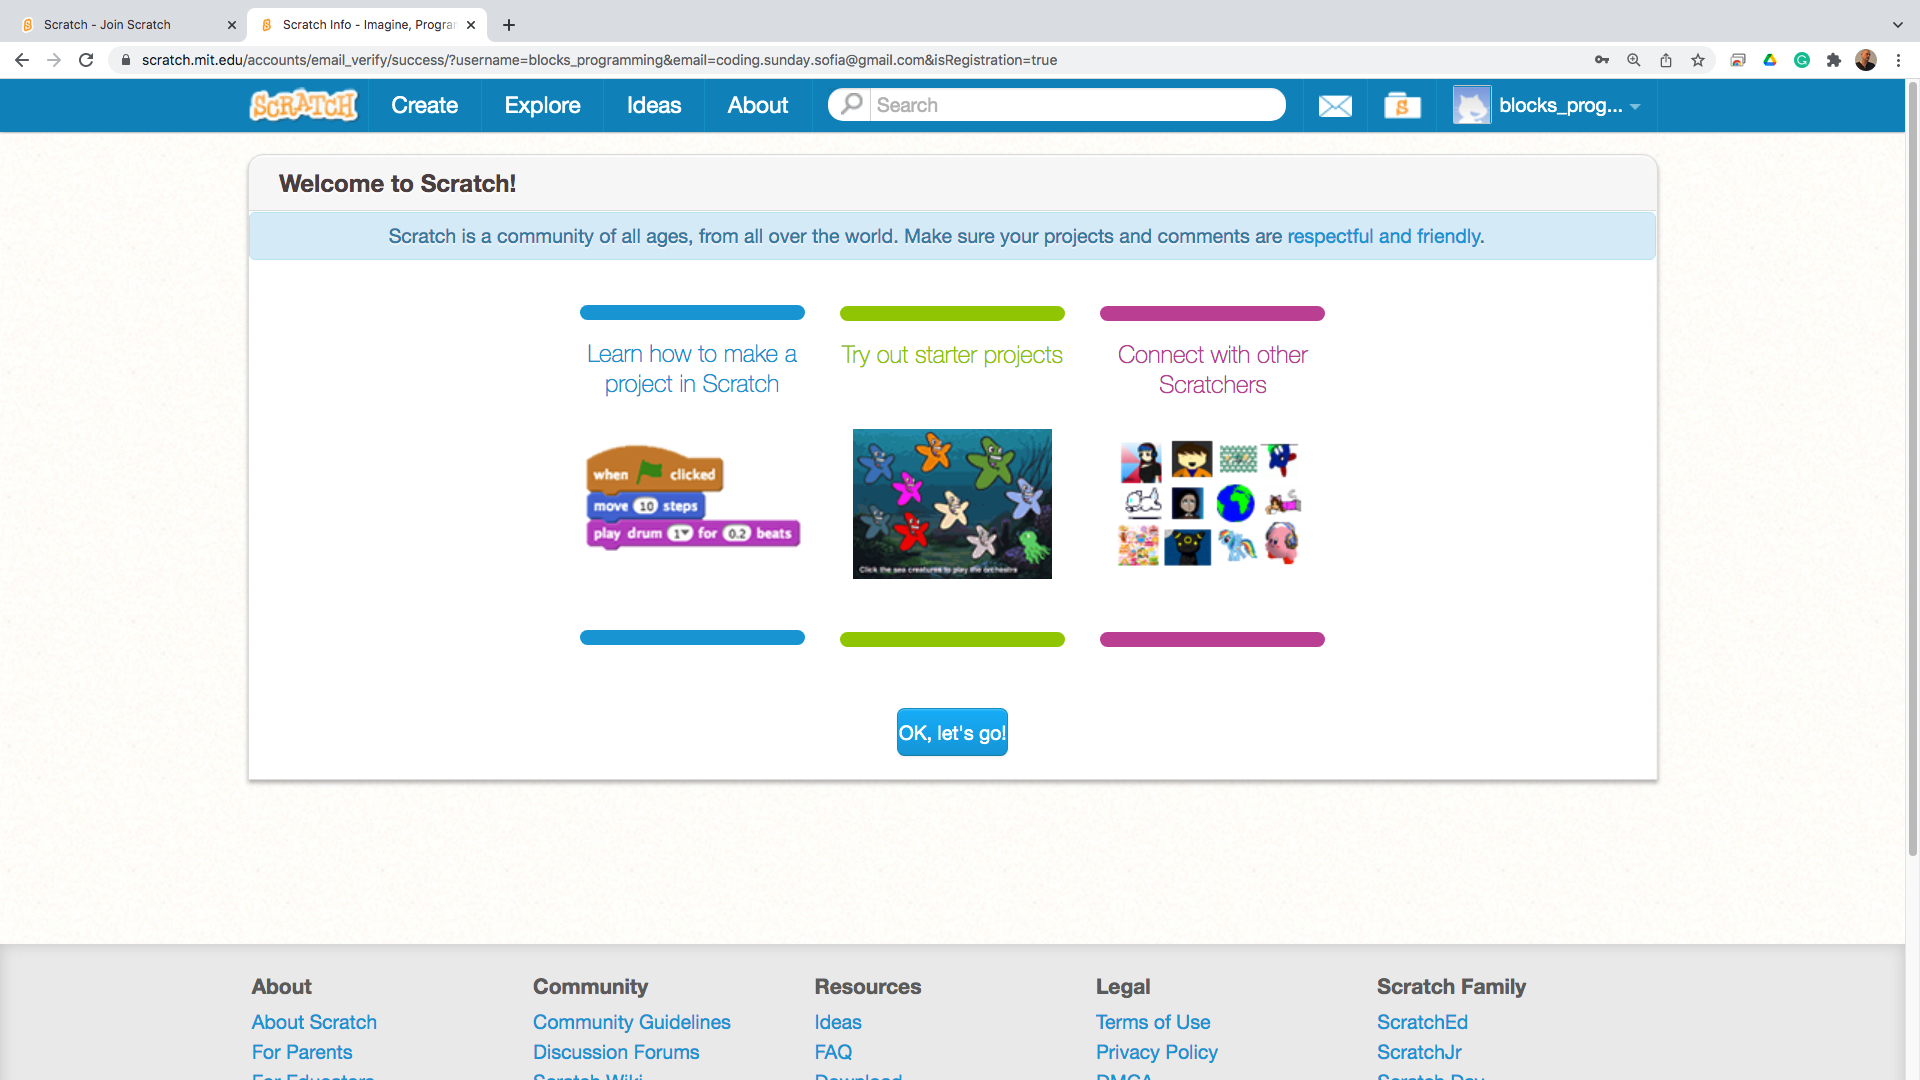
\includegraphics[width=1.0\linewidth,height=0.5\linewidth]{fig0009.png}
  \caption{Начален работен екран}
\label{fig0009}
\end{figure}

\section{Първи стъпки в App Inventor}

